% Part: biographies 
% Chapter: ernst-zermelo 
% Section: biography
\documentclass[../../../include/open-logic-section]{subfiles}

\begin{document}

\olfileid{bio}{erz}{bio} 
\olsection{Biography}
\begin{figure}[h!] 
\centering
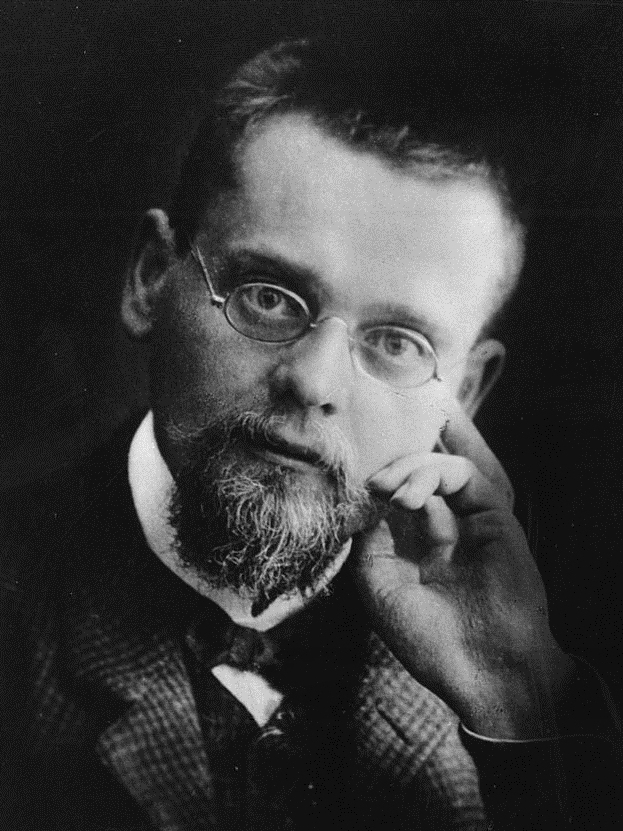
\includegraphics[scale=1]{ernst-zermelo.jpg} 
\caption{Ernst Zermelo. Photo Credit: Wikimedia Commons.} 
\end{figure}

Ernst Zermelo was born on July 27, 1871 in Berlin, Germany. He had five
sisters, though his family suffered from poor health and only three made it
to adulthood. His parents also passed away when he was young, leaving him
and his sibilings orphans when he was seventeen. Although known as a
mathematician, Zermelo had an interest in the arts, and especially in
poetry \citep[5]{Ebbinghaus2015}. He was known for being sharp, witty, and
critical. His most celebrated achievments include the intruduction of the
axiom of choice (in 1904), and his axiomatization of set theory (in 1908)
\citep[3]{Ebbinghaus2010}.

Zermelo's interests at univeristy were varied. He took courses in physics,
mathematics, and philosophy. Under the supervision of Hermann Schwarz,
Zermelo completed his dissertation \emph{Untersuchungen zur
Variations-Rechnung (Investigations In the Calculus of Variations)} in 1894
at the University of Berlin. In 1897, he decided to pursue more studies at
the Univeristy of G\"{o}ttigen where he was heavily influenced by the
foundational work of David Hilbert. In 1899 he became eligible for
professorship, but did not get one until eleven years later - possibly due
to his strange demeanour and "nervous haste" \citep[15]{Ebbinghaus2010}.

Zermelo finally recieved a paid professorship at the University of Zurich
in 1910, but was forced to retire in 1916 due to tuburculosis. After his
recovery, he was given an honourary professorship at the University of
Freiburg in 1921. During this time he worked on foundational mathematics.
He became irritated with the works of Thoraf Skolem and Kurt G\"{o}del,
even criticizing their approaches in his papers \citep[31]{Ebbinghaus2010}.
He was dismissed of his position at Freiburg in 1935, due to his
unpopularity and resistance to Hitler's rise to power in Germany
\citep[32]{Ebbinghaus2015}.
 
The later years of Zermelo's life were marked by isolation. In 1935, after
being let go from his position at Freiburg, he no longer pursued
mathematics. He moved to the country where he lived modestly. He married in
1944, and his wife was responsible for providing for them, as Zermelo was
going blind. He lost his sight completely by 1951. He passed away in
G\"{u}nterstal, Germany on May 21, 1953. 

\begin{reading}

\begin{itemize} 
\item A full biography of Zermelo is available by \citet{Ebbinghaus2015}.

\item Zermelo's collected works, including his writing on physics, are 
available in english translation. See \citet{Ebbinghaus2010,Ebbinghaus2013}.

\item Zermelo's seminal 1904 and 1908 papers are available to read in the
original german \citep{Zermelo1904,Zermelo1908}, and in english translation
 \citep{Ebbinghaus2013}.

\end{itemize}
 \end{reading}
\end{document}
